\subsection{Formulation of the problem}
	The initial velocity at the entrance to the channel is $U_0 = 0.29$ m/s. Turbulence intensity 5\%. At the exit from the channel, the condition of equality to zero of the derivative along the normal to the boundary is set. The no-flow and no-slip boundary conditions are set for the wall. This is expressed by the equality to zero of the normal and tangential velocity components.
	\begin{equation}
		v \cdot n = 0 \qquad v \cdot \tau = 0
	\end{equation}
	Here $n$ and $\tau$ are the unit vectors of the normal and tangent to the channel surface. The boundary conditions for the pressure are set by discretizing the equation for the change in momentum in the projection onto the normal to the wall.
	
	The wall restrains the growth of small eddies and changes the mechanism of energy exchange between resolvable and insoluble turbulence scales. In this case, the number of grid nodes required to calculate the flow in the boundary layer increases to a value characteristic of DNS. In order to reduce the consumption of computing resources and take into account the influence of various factors, such as surface roughness, the near-wall function method and various models of the turbulent boundary layer are used\cite{Cabot2000}.
	
	For non-stationary calculations, the condition of convective transport (non-reflecting boundary conditions) is applied. The mass flow at the inlet is equal to the mass flow at the exit from the computational domain.
	\begin{equation}
		\frac{\partial f}{\partial t} + U_0\frac{\partial f}{\partial n} = 0
	\end{equation}

\subsection{Visualization of the task}
	To construct the channel geometry and create a grid model, the built-in Ansys software tools were used. It provides a versatile, high performance, automated, intelligent meshing solution that generates the most appropriate model for accurate and efficient physics solutions -- from simple automatic meshing to complex, more hybrid and detailed meshing.
\subsubsection{Channel geometry}
	The object of study is a turbulent boundary layer in a channel. The channel is divided into two parts. The first part is a narrowing from 369.5$\times$149.8 mm at the beginning to 124$\times$50 mm. The length of this section is 396 mm. It allows you to significantly increase the flow rate of the liquid. The second part is straight, 1100 mm long.
	\begin{figure}[H]
		\centering
		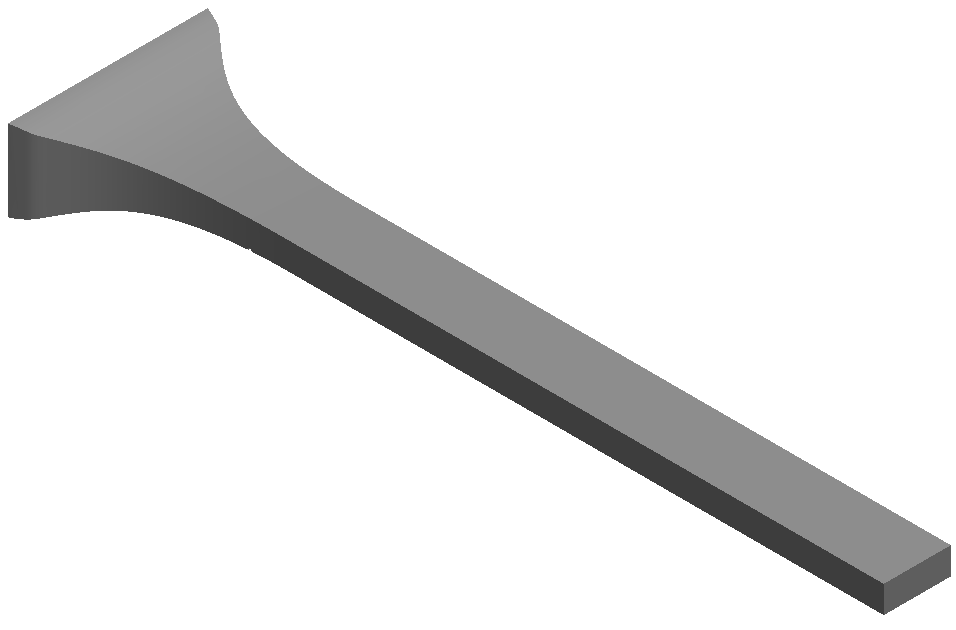
\includegraphics[width=0.7\linewidth]{../Assets/ВидКанала1}
		\caption{\footnotesize{General view of the channel}}
		\label{fig:channelview}
	\end{figure}
	At a distance of 323.9 mm from the entrance to the channel, at the base there is a cutout representing a wire with a radius of 2.1 mm and a height of 1.98 mm. This barrier creates a turbulent state.
	\begin{figure}[H]
		\centering
		
\includegraphics[width=0.5\linewidth]{../Assets/ВидКанала4}
		\caption{\footnotesize{View of the barrier in the channel}}
		\label{fig:vortexgeneratorview}
	\end{figure}
\subsubsection{Building a grid model}
	The most important part of any numerical simulation is the creation of a sufficiently detailed grid model. The accuracy of the results obtained depends on its quality. In addition, it requires a finer division for the boundary layer than for the main part of the channel, since the main processes of vortex formation occur precisely there.
	
	\begin{figure}[H]
		\centering
		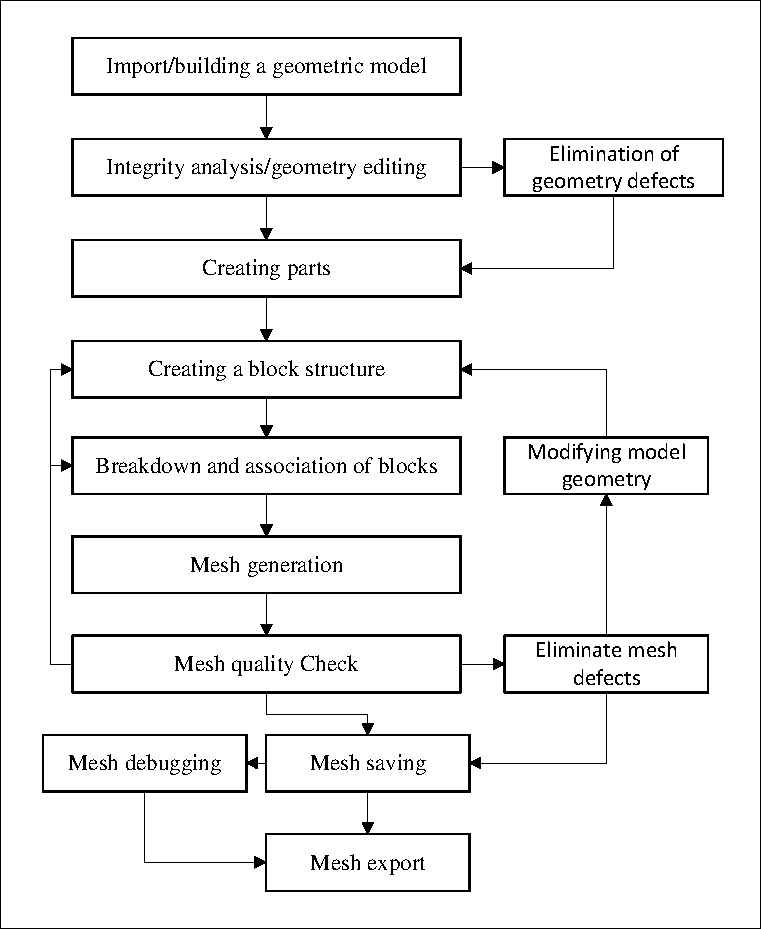
\includegraphics[width=0.7\linewidth]{../Assets/СхемаСозданияСеткиEN}
		\caption{\footnotesize{The scheme of work on the grid model}}
		\label{fig:meshScheme}
	\end{figure}
	The figure \ref{fig:meshScheme} shows a schematic plan for generating a mesh. This method is the most optimal for building a sufficiently high-quality grid model. Dividing the geometry into parts allows you to speed up the construction by parallel distribution of calculations (one core is allocated for each part). In addition, disabling the multithreading mode (one physical core is divided into two virtual ones) for the processor increases performance, since all the power of the core is used, and not half of it.
	
	There are several methods for modeling mesh models in Ansys that can be used depending on the type and size of the model.
	
	The first is the spatial partitioning method, which is often used to model rigid bodies. This method consists of breaking an object into smaller elements called leaf elements. Each finite element is then approximated with simpler shapes such as triangles or rectangles to create a mesh.
	
	The second is a node-based mesh generation method. In this method, the model is represented as a set of nodes connected by lines or surfaces. The mesh is then built based on this structure.
	
	The third is the multiple division method. This method is often used to model spatial objects such as aircraft or cars. It consists in breaking the object into smaller blocks and then dividing each block into even smaller blocks. Each block is then approximated with simpler shapes to create a mesh.
	
	\begin{figure}[H]
		\centering
		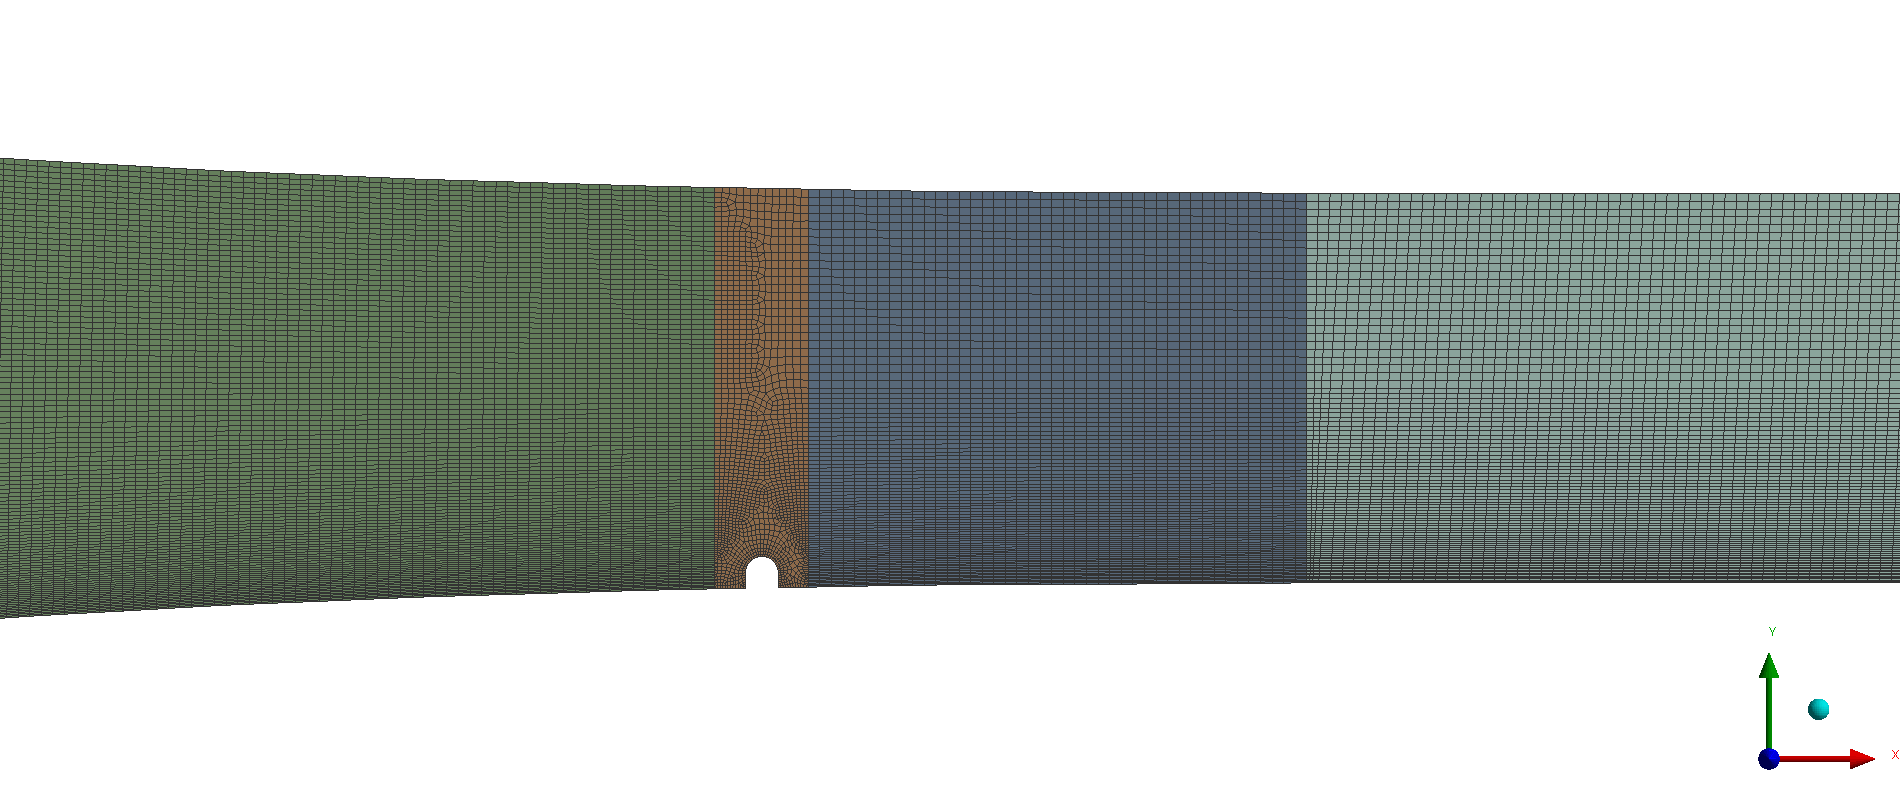
\includegraphics[width=1\linewidth]{../Assets/Mesh1}
		\caption{\footnotesize{Mesh}}
		\label{fig:mesh1}
	\end{figure}
	Using the plan and construction methods mentioned above, a grid model was built. With this grid, it was possible to achieve the optimal result for calculations. The channel was divided into 4 parts. The first part is the entrance to the canal, the second is the section with a barrier, the third is to the end of the narrowing, the fourth is the straight section of the canal. The grid model consists of 51397337 nodes and 12665608 elements.
	
\subsection{Problem calculation}
	Ansys Fluent is a general-purpose computational fluid dynamics (CFD) software used to model fluid flow, heat and mass transfer, chemical reactions, and more. Fluent offers a modern, user-friendly interface that streamlines the CFD process from pre- to post-processing within a single window workflow. Fluent is known for its advanced physics modeling capabilities, which include turbulence modeling, single and multiphase flows, combustion, battery modeling, fluid-structure interaction, and much more. Also known for its efficient HPC scaling, large models can easily be solved in Fluent on multiple processors on either CPU or GPU. Multiple solver options are available, including pressure-based and density-based CPU solvers to cover low-speed to hypersonic flows and a pressure-based native GPU solver.
	
	Let's move on to preparing for the calculations. Water was used as a liquid with the following characteristics: $\rho = 998.2$ $kg/m^3$ and $\nu = 0.001003$ $kg/m\cdot s$. For the subgrid model of the LES method, the WALE model was used with the coefficient $C_w = 0.325$. The main advantages of this model:
	\begin{itemize}
		\item the spatial operator contains both local deformations and rotational velocities. Thus, all turbulence structures related to the dissipation of kinetic energy are calculated by this model;
		\item the turbulent viscosity tends naturally to zero near the wall, so that neither a constant (dynamic) adjustment nor a damping function is required to calculate wall-bounded flows;
		\item the model gives zero turbulent viscosity in pure shear. Thus, it can reproduce the process of transition from laminar to turbulent flow due to the growth of linear unstable regimes.
	\end{itemize}
	In addition, the WALE model is invariant to any translation or rotation of coordinates, and only local information is required (no check-filter operation and no knowledge of nearest points in the grid), so it is well suited for LES in complex geometries\cite{Nicoud1999}.
	
	Discretization in the space produces a system of ordinary differential equations for unsteady problems and algebraic equations for steady problems. Implicit or semi-implicit methods are generally used to integrate the ordinary differential equations, producing a system of nonlinear algebraic equations. Applying a Newton or Picard iteration produces a system of linear equations which is nonsymmetric in the presence of advection and indefinite in the presence of incompressibility.
	
	The SIMPLEC algorithm was used as a solution method. It is a semi-implicit method for consistent pressure related equations. This schema is a modified form of the SIMPLE method. His algorithm was developed by Van Doormal and Raithby in 1984. In it, by changing the definition of the coefficients of the pressure correction equation, the effects of discarding neighboring grid velocity corrections are partially compensated (second approximation in the SIMPLE algorithm)\cite{Sun2008}.
	
	Some other parameters related to the calculation of equations:
	\begin{table}[H]
		\begin{center}
			\begin{tabular}{|c|c|}
				\hline
				Parameters & Method\\
				\hline
				Gradient & Least squares cell based\\
				\hline
				Pressure & Second order\\
				\hline
				Momentum & Bounded central differencing\\
				\hline
				Time & Bounded second order implicit\\
				\hline
			\end{tabular}
		\end{center}
		\caption{\footnotesize{Solver options}}
	\end{table}
	With the settings and parameters described above, the calculation was launched in ANSYS FLUENT. The time step size is $\Delta t = 0.001 s$, their number is $s_t = 10000$. $s_i = 50$ iterations were calculated for each step. This is 10s of real time.